\documentclass{article}

% PREAMBOLO
\usepackage[utf8]{inputenc}
\usepackage[italian]{babel}
\usepackage{amsmath}
\usepackage{amsfonts}
\usepackage{amssymb}
\usepackage{geometry}
\usepackage{graphicx}
\geometry{a4paper, top=3cm, bottom=3cm, left=3cm, right=3cm}
\usepackage{booktabs} % Per tabelle eleganti
\usepackage[hidelinks]{hyperref} % Per link cliccabili
\usepackage{caption} % Per impostazioni delle caption di tabelle e figure
\captionsetup{font=it} % Caption in corsivo

\begin{document}


\noindent\normalsize Relazione di progetto per il corso di: \hfill \textbf{Gruppo n. 12}\\
\textbf {Introduzione alla Data Science} \hfill Nicoletta Aloisi matr. 1216124\\
\textbf {e al Pensiero Computazionale} \hfill Erika Avdiaj matr. 1226030\\
\normalsize A.A. 2025/2026 \hfill Giannalisa Romeo matr. 1216078\\
\normalsize docente: Francesco Poggi\\
\\ \\
\noindent
\huge\textbf{Analisi del Turnover del Personale} \\  
\normalsize Previsione dell'abbandono dei dipendenti tramite tecniche di Machine Learning
\\ \\


\section{Introduzione}
Il presente studio nasce con un obiettivo conoscitivo ed applicativo fondamentale: analizzare un dataset aziendale per comprendere quanti dipendenti interrompano il proprio rapporto lavorativo con questa azienda e, soprattutto, identificare le motivazioni che spingono a compiere questa scelta.  \\
Per raggiungere un adeguato livello di robustezza metodologica e scientifica, il percorso del nostro gruppo è stato strutturato secondo una divisione del lavoro sequenziale articolato in cinque fasi:
\begin{description}
    \item[Fase 1: Setup del progetto e repository GitHub]\mbox{}\\Questa fase preliminare è stata dedicata all'architettura logica e infrastrutturale. Si è provveduto alla configurazione dell'ambiente di lavoro cooperativo su GitHub, strutturando le directory di progetto (data, notebooks, figures, report) e implementando un controllo di versione volto a garantire la tracciabilità e la riproducibilità del codice.

  \item[Fase 2: Descrizione e comprensione del dataset]\mbox{}\\ Incentrata sulla comprensione strutturale, questa fase ha previsto la verifica dell'integrità qualitativa dei dati e l'identificazione della loro natura statistica, ponendo le basi per la formulazione delle nostre ipotesi di ricerca.

  \item[Fase 3: Analisi esplorativa e visualizzazione]\mbox{}\\In questa fase, l'indagine si sposterà sullo studio grafico e statistico. Attraverso diversi grafici (\textit{scatterplot}, \textit{boxplot}, \textit{heatmap}, \textit{barplot}, ecc.), cercheremo di far emergere i primi pattern significativi legati all'\textit{attrition}.

  \item[Fase 4: Modellazione]\mbox{}\\In questa fase le evidenze empiriche verranno convertite in modelli matematico-statistici. Verranno addestrati differenti classificatori di Machine Learning (come la Regressione Logistica, il \textit{k}-Nearest Neighbors e i Random Forest) per stimare la probabilità di abbandono.


 \item[Fase 5: Valutazione e interpretazione dei risultati]\mbox{}\\La fase conclusiva del progetto riguarderà il monitoraggio comparativo delle performance dei modelli tramite metriche quali Accuratezza, Precisione, \textit{Recall}, F1-Score. Questa fase ospiterà una serie di riflessioni critiche esaminandone i punti di forza, i limiti intrinseci, il livello di interpretabilità dei parametri e la tipologia di errori commessi (analizzando l'impatto dei falsi positivi e dei falsi negativi). Verranno inoltre valutati il costo computazionale richiesto e la robustezza generale degli algoritmi di fronte allo sbilanciamento dei dati, con il fine ultimo di identificare dei pattern predittivi per la prevenzione del turnover.
\end{description}

\newpage
\section{Descrizione e comprensione del dataset}
Nella seconda fase del progetto abbiamo studiato la struttura del dataset \texttt{Employee\_Attrition}. Utilizzando i comandi Python \texttt{emp.shape} ed \texttt{emp.dtypes}, abbiamo visto che la matrice dei dati contiene \textbf{1470 righe} (osservazioni) e \textbf{35 colonne} (le variabili), divise tra \textbf{26 variabili numeriche} e \textbf{9 categoriche} (testuali). \\
La nostra variabile obiettivo (Target) è \textbf{\texttt{Attrition}}, una variabile binaria che indica se il dipendente ha lasciato l'azienda (\texttt{Yes}) o è rimasto (\texttt{No}). \\
Analizzando le frequenze abbiamo scoperto un forte sbilanciamento dei dati (\textit{class imbalance}):
\begin{itemize}
    \item \textbf{Classe No:} 1233 dipendenti (83,88\%)
    \item \textbf{Classe Yes:} 237 dipendenti (16,12\%)
\end{itemize}

\noindent Questo sbilanciamento è un elemento centrale: un modello banale che dice sempre \texttt{"No"} indovinerebbe l'84\% delle volte (\textit{accuracy}), ma sarebbe inutile perché non troverebbe nessun dipendente che sta per andarsene. Per questo motivo, nelle fasi successive guarderemo particolarmente \textit{precision}, \textit{recall} e \textit{F1-score}.\\

\noindent In seguito abbiamo controllato la qualità dei dati con il comando \texttt{emp.isnull().sum()}, confermando che il dataset è integro e presenta lo \textbf{0\% di valori mancanti}. Tramite la funzione \texttt{emp.describe()} abbiamo estratto cinque statistiche chiave:
\begin{enumerate}
    \item \textbf{Età (\texttt{Age}):} La media è di circa 37 anni.
    \item \textbf{Distanza da casa (\texttt{DistanceFromHome}):} La media è di 9,2 km mentre la mediana è di 7 km; lo scostamento indica che ci sono alcuni dipendenti che vivono piuttosto lontani dal posto di lavoro.
    \item \textbf{Stipendio mensile (\texttt{MonthlyIncome}):} La media (6503) è molto più alta della mediana (4919); questo significa che la distribuzione è sbilanciata verso l'alto a causa di pochi manager che guadagnano cifre molto elevate.
    \item \textbf{Anzianità (\texttt{TotalWorkingYears} e \texttt{YearsAtCompany}):} I dipendenti hanno in media 11,3 anni di esperienza lavorativa totale, ma sono in questa azienda da circa 7 anni (con una mediana di soli 5 anni); la maggior parte dei dipendenti ha esperienza pregressa, ma è in azienda da relativamente poco tempo.
    \item \textbf{Soddisfazione (\texttt{JobSatisfaction}):} Il voto medio è di 2,7 su una scala da 1 a 4, indicando una soddisfazione moderata.
\end{enumerate}

\noindent Basandoci sulle caratteristiche dei dati, abbiamo formulato varie ipotesi di ricerca: dall’impatto dei fattori logistici ed economico-generazionali, alle trasferte e agli straordinari. Nelle fasi successive (grafici e modelli), vedremo se queste ipotesi verranno confermate o smentite. Abbiamo dunque elaborato tre riflessioni critiche:

\begin{itemize}
    \item \textbf{Gestione del Class Imbalance:} Dato il forte sbilanciamento del target \texttt{Attrition} (84\% \texttt{No}, 16\% \texttt{Yes}), in Fase 3 dovremo analizzare le distribuzioni condizionate specificamente sulla classe minoritaria (\texttt{"Yes"}) per evitare che i comportamenti dei dipendenti rimasti in azienda nascondano i segnali di chi abbandona. Inoltre, in Fase 4 questa asimmetria ci costringerà a declassare in parte l'importanza dell'\textit{accuracy}, facendo attenzione più a \textit{precision}, \textit{recall} e \textit{F1-score}.
    
    \item \textbf{Asimmetria e presenza di Outlier:} Il fatto che variabili chiave come \texttt{MonthlyIncome} e \texttt{DistanceFromHome} presentino una media superiore alla mediana è segnale di distribuzioni asimmetriche e della presenza di valori estremi (\textit{outlier}), come nel caso dei pochissimi manager con stipendi molto elevati. Nella Fase 3 sfrutteremo grafici come i \textit{boxplot} per isolare visivamente questi \textit{outlier}.
    
    \item \textbf{Rimozione di Feature degenerate e identificative:} Le colonne \texttt{EmployeeCount}, \texttt{Over18} e \texttt{StandardHours} assumono lo stesso identico valore per tutti i dipendenti, non apportando alcuna informazione discriminante per separare le due classi del target. Allo stesso modo, \texttt{EmployeeNumber} rappresenta un identificativo univoco privo di significato predittivo. Per evitare di introdurre rumore statistico, queste quattro variabili verranno rimosse.
\end{itemize}


\section{Metodologia}
\label{sec:metodologia}

\subsection{Analisi esplorativa}
\label{sec:metodologia-eda}

L'analisi esplorativa ha seguito uno schema sistematico: per ciascuna domanda di ricerca è stata individuata una visualizzazione o statistica appropriata, i dati sono stati manipolati per rispondere alla domanda (filtri, aggregazioni, tabelle di contingenza) e infine è stata formulata un'interpretazione basata sull'evidenza osservata. Sono stati impiegati diversi strumenti grafici della libreria \texttt{seaborn}: \emph{heatmap} triangolare per le correlazioni tra variabili numeriche, \emph{boxplot} e \emph{violin plot} per confrontare le distribuzioni di variabili continue tra gruppi, \emph{barplot} per confrontare percentuali di abbandono tra categorie, e uno \emph{scatterplot} per esplorare la relazione tra esperienza lavorativa e reddito. In tutti i confronti si è tenuto conto della natura osservazionale del dataset: le associazioni individuate non implicano un nesso causale.

\subsection{Preparazione dei dati per la modellazione}
\label{sec:metodologia-prep}

Prima di addestrare i modelli predittivi il dataset è stato sottoposto a una fase di pulizia e trasformazione.

\paragraph{Rimozione delle feature non informative.} Sono state eliminate le variabili \texttt{EmployeeCount}, \texttt{Over18} e \texttt{StandardHours}, che assumono lo stesso valore per tutte le 1470 osservazioni (varianza nulla), e \texttt{EmployeeNumber}, un identificativo univoco privo di potere predittivo. Sono state inoltre rimosse le variabili derivate \texttt{AgeGroup} e \texttt{IncomeGroup}, create in Fase 3 a fini esplorativi, in quanto ridondanti rispetto a \texttt{Age} e \texttt{MonthlyIncome}.

\paragraph{Codifica delle variabili categoriche.} La variabile target \texttt{Attrition} è stata ricodificata in formato binario (\emph{No} $ = 0$, \emph{Yes} $ = 1$). Le variabili categoriche predittive (\texttt{BusinessTravel}, \texttt{Department}, \texttt{EducationField}, \texttt{JobRole}, \texttt{MaritalStatus}, \texttt{Gender}, \texttt{OverTime}) sono state trasformate in numeriche tramite \texttt{pd.get\_dummies}, con \texttt{drop\_first=True}, ottenendo un dataset finale di 1470 osservazioni e 45 colonne (44 variabili predittive più il target).

\paragraph{Suddivisione training/test.} Il dataset è stato diviso in un insieme di addestramento (80\%, 1176 osservazioni) e uno di test (20\%, 294 osservazioni), utilizzando la stratificazione rispetto alla variabile target per preservare in entrambi gli insiemi la proporzione originaria delle classi (84\% \emph{No}, 16\% \emph{Yes}), coerentemente con lo sbilanciamento rilevato di analisi del dataset.


\paragraph{Standardizzazione.} Le variabili numeriche sono state standardizzate secondo la formula
\begin{equation}
\mu = \frac{1}{n}\sum_{i=1}^{n} x_i, \qquad \sigma = \sqrt{\frac{1}{n}\sum_{i=1}^{n}(x_i - \mu)^2}, \qquad z_i = \frac{x_i - \mu}{\sigma}
\label{eq:standardizzazione}
\end{equation}
dove $\mu$ e $\sigma$ sono, rispettivamente, media e deviazione standard calcolate esclusivamente sul training set ($n=1176$ osservazioni) e successivamente applicate anche al test set, per evitare fughe di informazione (\emph{data leakage}). La standardizzazione è necessaria per il k-NN, sensibile alla scala delle variabili nel calcolo delle distanze, e migliora la stabilità numerica della Regressione Logistica; non è invece richiesta per la Random Forest, un modello basato su alberi e quindi invariante rispetto alla scala delle feature.

\subsection{Modelli di apprendimento supervisionato}
\label{sec:metodologia-modelli}

In Fase 3, a scopo puramente esplorativo, è stata stimata una regressione lineare semplice tra gli anni di esperienza lavorativa e il reddito mensile, secondo il modello
\begin{equation}
\hat{y} = ax + b
\label{eq:reg_lineare}
\end{equation}
con $x = \texttt{TotalWorkingYears}$ e $\hat{y} = \texttt{MonthlyIncome}$. La stima ha prodotto $a = 467{,}66$ e $b = 1227{,}94$, evidenziando una relazione positiva tra le due variabili. Si sottolinea che questo modello ha finalità descrittiva e non è utilizzato per predire l'abbandono: il problema di classificazione binaria della variabile \texttt{Attrition} è stato affrontato nella fase di modellazione con tre modelli distinti, riassunti in Tabella~\ref{tab:modelli}.


\begin{table}[h]
\centering
\small %riducendo il font la tabella resta della stessa larghezza del paragrafo
\begin{tabular}{l l c l}
\hline
\textbf{Modello} & \textbf{Tipo} & \textbf{Standardizzazione} & \textbf{Iperparametri} \\
\hline
Regressione Logistica & Lineare & Sì & default (\texttt{scikit-learn}) \\
k-Nearest Neighbors & Non lineare & Sì & $k = 5$ \\
Random Forest & Non lineare & No & \texttt{n\_estimators=200}, \texttt{random\_state=42} \\
\hline
\end{tabular}
\caption{Sintesi dei modelli di classificazione impiegati nella fase di modellazione, con relativi requisiti di preprocessing e iperparametri.}
\label{tab:modelli}
\end{table}

\noindent I tre modelli si distinguono per il meccanismo di classificazione: la Regressione Logistica stima una probabilità tramite una combinazione lineare delle feature; il k-NN classifica in base alla classe maggioritaria tra i $k=5$ vicini più prossimi; la Random Forest aggrega il voto di 200 alberi decisionali.


\subsection{Metriche di valutazione}
\label{sec:metodologia-metriche}

Data la classe \emph{Yes} come classe positiva, i modelli sono stati valutati sul test set tramite le metriche standard per la classificazione binaria: \emph{accuracy}, \emph{precision}, \emph{recall} e \emph{F1-score}, calcolate a partire dai veri positivi, veri negativi, falsi positivi e falsi negativi prodotti da ciascun modello. Data la natura sbilanciata del target, un modello che predicesse sempre la classe maggioritaria otterrebbe comunque un'accuracy dell'84\% senza alcuna utilità pratica: per questo motivo precision, recall e F1-score sulla classe \emph{Yes}, insieme alla matrice di confusione, sono state considerate le metriche più informative ai fini della valutazione. In particolare, in un contesto di prevenzione del turnover un falso negativo (un dipendente a rischio non individuato dal modello) rappresenta l'errore più critico, poiché comporta la mancata attivazione di eventuali interventi da parte delle Risorse Umane.

\newpage

\section{Risultati}
\label{sec:risultati}

\subsection{Evidenze principali dell'analisi esplorativa}
\label{sec:risultati-eda}

L'analisi esplorativa ha evidenziato pattern coerenti riconducibili a tre dimensioni principali.

\paragraph{Fattori economici.} Il reddito mensile è risultato uno dei fattori più associati all'abbandono: a parità di genere, i dipendenti con reddito $\leq 5.000$ presentano tassi di attrition nettamente superiori rispetto a quelli con reddito più elevato, mentre le differenze tra uomini e donne risultano marginali. Il reddito cresce inoltre in modo sistematico con il \texttt{JobLevel}, e l'effetto protettivo di un reddito più alto è particolarmente marcato ai livelli professionali superiori (Figura~\ref{fig:heatmap}).

\paragraph{Età e reddito.} La distribuzione del reddito differisce nettamente tra i dipendenti che hanno lasciato l'azienda e quelli rimasti, in tutte le fasce d'età (Figura~\ref{fig:violin}): chi resta presenta redditi più elevati e distribuzioni più ampie, con differenze particolarmente marcate nelle fasce 41-50 e 51+. Questo suggerisce che l'interazione tra età e reddito è potenzialmente più informativa del solo effetto dell'età.

\paragraph{Carico di lavoro e mobilità.} Gli straordinari (\texttt{OverTime}) e la frequenza delle trasferte (\texttt{Business Travel}) sono emersi come i fattori di rischio più marcati, con un effetto particolarmente pronunciato tra i profili junior che svolgono straordinari; le trasferte frequenti aumentano l'attrition soprattutto tra i dipendenti single.

\paragraph{Esperienza e stabilità.} Una minore anzianità in azienda, una minore esperienza lavorativa complessiva e una maggiore distanza da casa sono risultate associate a una maggiore probabilità di abbandono.

\begin{figure}[ht]
\centering
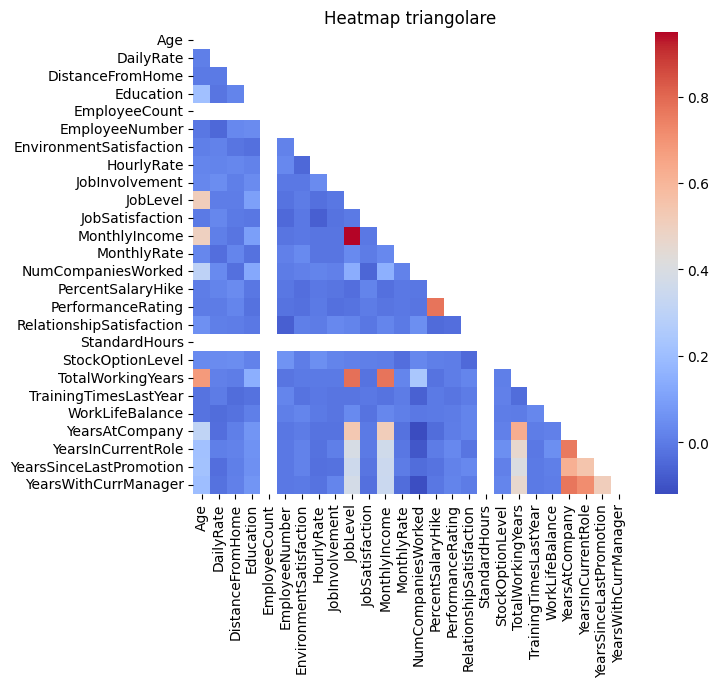
\includegraphics[width=0.75\textwidth]{figures/heatmap_correlazioni.png}
\caption{Heatmap triangolare delle correlazioni tra le variabili numeriche del dataset.}
\label{fig:heatmap}
\end{figure}

\begin{figure}[ht]
\centering
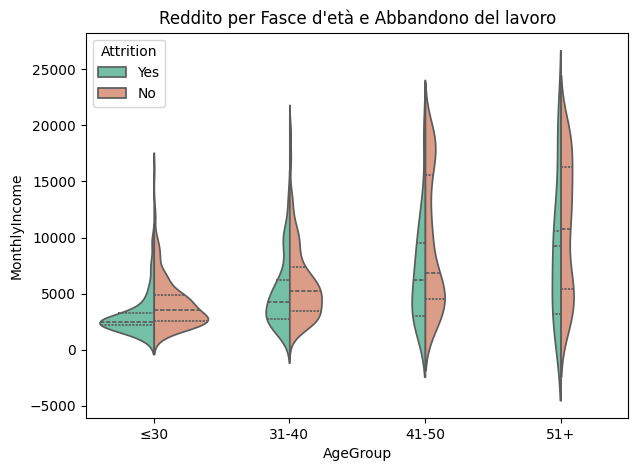
\includegraphics[width=0.9\textwidth]{figures/violinplot_age_income_attrition.png}
\caption{Distribuzione del reddito mensile per fascia d'età e Attrition.}
\label{fig:violin}
\end{figure}

\subsection{Confronto tra i modelli}
\label{sec:risultati-modelli}

La Tabella~\ref{tab:confronto_modelli} riporta le metriche di valutazione (Sezione~\ref{sec:metodologia-metriche}) calcolate sul test set per i tre modelli addestrati in Fase 4.

\begin{table}[h]
\centering
\begin{tabular}{l c c c c}
\hline
\textbf{Modello} & \textbf{Accuracy} & \textbf{Precision} & \textbf{Recall} & \textbf{F1-score} \\
\hline
Regressione Logistica & 0,86 & 0,62 & 0,34 & 0,44 \\
k-NN ($k=5$)          & 0,85 & 0,62 & 0,11 & 0,18 \\
Random Forest         & 0,84 & 0,46 & 0,13 & 0,20 \\
\hline
\end{tabular}
\caption{Confronto delle metriche di valutazione (classe positiva \emph{Yes}) tra i tre modelli sul test set (294 osservazioni).}
\label{tab:confronto_modelli}
\end{table}

\noindent Le accuracy dei tre modelli sono molto simili tra loro (84-86\%) e vicine al livello base dell'84\%, ottenibile predicendo sempre la classe maggioritaria (Sezione~\ref{sec:metodologia-metriche}): l'accuracy da sola, quindi, non è sufficiente a discriminare tra i modelli. Le differenze sostanziali emergono invece su precision, recall e F1-score relativi alla classe \emph{Yes}, come confermato dalla matrice di confusione (Figura~\ref{fig:confusion_matrices}).

\noindent La Regressione Logistica identifica correttamente 16 dei 47 dipendenti che hanno effettivamente lasciato l'azienda (recall $=0,34$), un valore nettamente superiore rispetto al k-NN (5 su 47, recall $=0,11$) e alla Random Forest (6 su 47, recall $=0,13$). Di conseguenza, la Regressione Logistica genera meno falsi negativi (31, contro 42 del k-NN e 41 della Random Forest): nel contesto applicativo del progetto, in cui un falso negativo corrisponde a un dipendente a rischio non intercettato, questo la rende il modello più utile ai fini decisionali, nonostante le tre accuracy siano pressoché equivalenti.
\newpage
\begin{figure}[h]
\centering
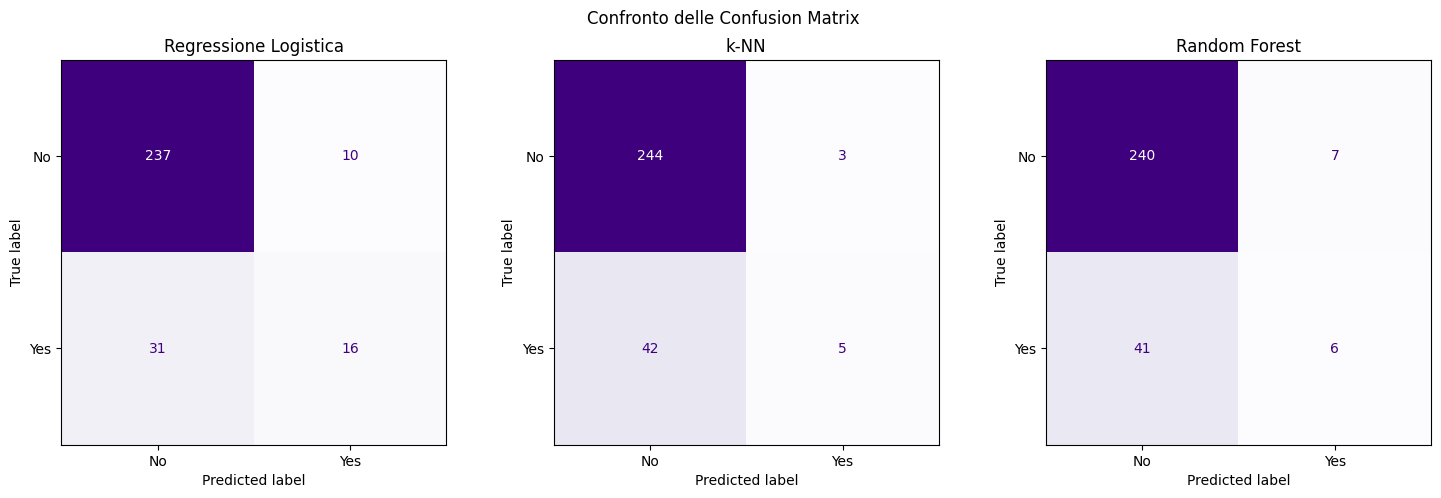
\includegraphics[width=\textwidth]{figures/confusion_matrices_confronto.png}
\caption{Matrici di confusione dei tre modelli sul test set (294 osservazioni: 247 \emph{No}, 47 \emph{Yes}).}
\label{fig:confusion_matrices}
\end{figure}

\subsection{Interpretabilità dei modelli}
\label{sec:risultati-interpretabilita}

L'analisi dei coefficienti della Regressione Logistica (Sezione~\ref{sec:metodologia-modelli}) permette di individuare i fattori più associati al rischio di abbandono. La Tabella~\ref{tab:coefficienti} riporta i cinque coefficienti più elevati (fattori di rischio) e i cinque più bassi (fattori protettivi).

\begin{table}[h]
\centering
\small
\begin{tabular}{l c l c}
\hline
\textbf{Fattore di rischio} & \textbf{Coeff.} & \textbf{Fattore protettivo} & \textbf{Coeff.} \\
\hline
OverTime (sì)                        & $+0,86$ & TotalWorkingYears        & $-0,56$ \\
BusinessTravel (frequenti)           & $+0,75$ & EnvironmentSatisfaction  & $-0,48$ \\
JobRole: Laboratory Technician       & $+0,71$ & JobSatisfaction          & $-0,42$ \\
YearsSinceLastPromotion              & $+0,53$ & Age                      & $-0,41$ \\
NumCompaniesWorked                   & $+0,49$ & YearsWithCurrManager     & $-0,40$ \\
\hline
\end{tabular}
\caption{Coefficienti della Regressione Logistica: primi 5 fattori di rischio e primi 5 fattori protettivi (feature standardizzate).}
\label{tab:coefficienti}
\end{table}

\noindent I segni dei coefficienti sono coerenti con quanto osservato in fase di esplorazione del dataset: gli straordinari e le trasferte frequenti risultano i principali fattori di rischio, mentre una maggiore anzianità lavorativa e una maggiore soddisfazione (ambientale e lavorativa) risultano protettive.

\noindent La Random Forest non produce coefficienti singoli ma una misura di \emph{feature importance}; le prime cinque variabili per importanza sono \texttt{MonthlyIncome}, \texttt{Age}, \texttt{TotalWorkingYears}, \texttt{DailyRate} e \texttt{MonthlyRate}. Da notare che \texttt{MonthlyIncome}, la più importante per la Random Forest, non compare tra i coefficienti principali della Regressione Logistica: un possibile effetto non lineare che il modello ad alberi coglie meglio.


\newpage
\section{Discussione}
 
\subsection{Convergenza tra analisi esplorativa e modellazione}
I risultati ottenuti nelle Fasi 3 e 4 mostrano coerenza interna.
Le variabili individuate come più associate all'abbandono durante l'analisi esplorativa (\texttt{OverTime}, \texttt{BusinessTravel}, \texttt{MonthlyIncome},
\texttt{YearsAtCompany} e \texttt{TotalWorkingYears}) compaiono puntualmente tra i coefficienti più significativi della Regressione Logistica
(Tabella~\ref{tab:coefficienti}) e tra le variabili a maggiore \emph{feature importance}
per la Random Forest. Questa convergenza rafforza l'affidabilità delle evidenze emerse e
suggerisce che i pattern individuati siano segnali robusti presenti nella struttura del dataset.
 
\subsection{L'inganno dell'accuracy e il ruolo del class imbalance}
Come anticipato in Fase 2, il forte sbilanciamento del target (84\% \emph{No},
16\% \emph{Yes}) rende l'accuracy una metrica fuorviante: un classificatore banale che
predice sempre la classe maggioritaria raggiungerebbe già l'84\% di accuracy senza
individuare alcun caso reale di abbandono. Le accuracy dei tre modelli (86\%, 85\%, 84\%)
sono fra loro molto simili e si avvicinano tutte a questa soglia di riferimento: le differenze sostanziali emergono solo guardando precision, recall e F1-score sulla classe \emph{Yes}, come riportato in Tabella~\ref{tab:confronto_modelli}.
 
\noindent È proprio su questa dimensione che la Regressione Logistica si distingue nettamente
(recall $= 0{,}34$, F1 $= 0{,}44$), mentre k-NN e Random Forest si fermano entrambi a
un recall di $0{,}11$ e producono 42 falsi negativi ciascuno contro i 31 della Regressione
Logistica, come visibile nelle matrici di confusione (Figura~\ref{fig:confusion_matrices}).
 
\subsection{Il costo degli errori nel contesto aziendale}
I due tipi di errore di classificazione non hanno lo stesso peso applicativo.
Un \textbf{falso positivo} comporta l'attivazione di un intervento di \emph{retention}
verso un dipendente che sarebbe comunque rimasto: un costo limitato e reversibile.
Un \textbf{falso negativo} è invece più grave, perché il modello non individua un
dipendente che lascerà davvero l'azienda, facendo perdere all'azienda
l'opportunità di intervenire tempestivamente.\\
 
\noindent In quest'ottica, la Regressione Logistica, pur non essendo il modello più ``potente''
in assoluto, rappresenta la scelta più indicata per questo obiettivo,
grazie al minor numero di falsi negativi e alla sua interpretabilità: i coefficienti permettono di comunicare le ragioni della previsione in modo comprensibile anche per un pubblico non tecnico.
 
\subsection{Limiti dell'analisi}
Occorre sottolineare che tutte le associazioni individuate --- sia nell'analisi esplorativa, sia attraverso i coefficienti della Regressione Logistica --- sono di natura \textbf{statistica e osservazionale}, e non devono essere interpretate come relazioni causali. Il fatto che chi fa straordinari abbandoni di più, ad esempio, non implica necessariamente che gli straordinari \emph{causino} l'abbandono: entrambi potrebbero essere effetti di un fattore sottostante non osservato, come un clima aziendale negativo o una cattiva gestione.

\newpage
\section{Conclusioni}
\label{sec:conclusioni}
Il progetto ha prodotto un'analisi del fenomeno dell'attrition
aziendale, integrando esplorazione dei dati, visualizzazione e modellazione predittiva
in un flusso di lavoro organizzato tramite GitHub e documentato nella presente relazione.
 
\paragraph{Sintesi per fase.}
\begin{itemize}
  \item \textbf{Fase 2:} sono state rimosse tre variabili costanti prive di contenuto
    informativo (\texttt{Employee Count}, \texttt{Over18}, \texttt{StandardHours})
    e l'identificativo \texttt{EmployeeNumber}. Il forte sbilanciamento del target
    (84\% \emph{No}, 16\% \emph{Yes}) è stato segnalato come vincolo metodologico
    centrale per le fasi successive.
 
  \item \textbf{Fase 3:} i dipendenti che svolgono straordinari presentano un tasso di
    attrition del 30\% contro il 10\% di chi non li svolge; redditi mensili bassi,
    trasferte frequenti, giovane età e poca anzianità aziendale risultano tutti
    associati a una maggiore probabilità di abbandono.
 
  \item \textbf{Fase 4:} la Regressione Logistica ha ottenuto le prestazioni migliori
    sulla classe minoritaria (recall $= 0{,}34$, F1 $= 0{,}44$), con un numero di
    falsi negativi inferiore rispetto a k-NN e Random Forest. I coefficienti confermano
    \texttt{OverTime} e \texttt{BusinessTravel} come principali fattori di rischio,
    e \texttt{TotalWorkingYears}, \texttt{EnvironmentSatisfaction} e
    \texttt{JobSatisfaction} come fattori protettivi (che trattengono i dipendenti in azienda).
 
  \item \textbf{Fase~5:} il confronto tra i modelli ha confermato che, in presenza di
    classi sbilanciate, il recall sulla classe minoritaria è la metrica più informativa
    ai fini decisionali, poiché il costo di un falso negativo supera quello di un
    falso positivo nel contesto aziendale.
\end{itemize}
 
\paragraph{Variabili chiave.}
Nel complesso, il rischio di attrition risulta principalmente associato a:
\texttt{Monthly Income}, \texttt{TotalWorkingYears}, \texttt{Age}, \texttt{OverTime},
\texttt{BusinessTravel}, \texttt{YearsWithCurrManager} e \texttt{YearsIn CurrentRole}.
Queste variabili sono le più utili per identificare i profili a rischio e orientare
eventuali interventi aziendali.
 
\paragraph{Implicazioni applicative.}
I risultati suggeriscono che politiche mirate alla riduzione degli straordinari, alla gestione delle trasferte, al miglioramento della soddisfazione lavorativa e ambientale, e alla stabilità del rapporto con il responsabile diretto potrebbero contribuire concretamente a ridurre il tasso di abbandono. Anche investimenti in formazione (\texttt{TrainingTimesLastYear}) e benefit economici (\texttt{StockOptionLevel}) mostrano un'associazione positiva con la fedeltà aziendale.
 
\section*{Dichiarazione sull'uso dell'Intelligenza Artificiale}
Nel corso del progetto è stato fatto uso di assistenti LLM, in particolare Claude, come supporto alla programmazione Python. L'utilizzo è avvenuto esclusivamente per suggerimenti
sintattici e strutturali; tutte le scelte analitiche, le interpretazioni dei risultati e i commenti critici sono stati elaborati autonomamente dal gruppo.
Di seguito si riportano i costrutti per i quali è stato richiesto supporto all'AI, con indicazione del contesto d'uso:
 
\begin{enumerate}
 
  \item \textbf{\texttt{.nunique()}} --- usato in Fase 2 per identificare le colonne
    con un unico valore distinto (variabili costanti), così da individuare ed eliminare
    \texttt{EmployeeCount}, \texttt{Over18} e \texttt{StandardHours}.
 
  \item \textbf{\texttt{.apply(lambda x: (x == 'Yes').mean())} con
    \texttt{.reset\_index(name='Attrition (\%)')}} --- usato in Fase 3 per calcolare
    la percentuale di attrition per ciascun gruppo (es.\ per livello professionale
    e presenza di straordinari).
 
  \item \textbf{\texttt{pd.get\_dummies(..., drop\_first=True)}} --- usato in Fase 4
    per applicare l'One-Hot Encoding alle variabili categoriche
    (\texttt{BusinessTravel}, \texttt{Department}, \texttt{EducationField},
    \texttt{JobRole}, \texttt{MaritalStatus}, \texttt{Gender}, \texttt{OverTime})
    prima dell'addestramento dei modelli.
 
  \item \textbf{\texttt{kind='barh'}} --- parametro di \texttt{pandas.DataFrame.plot()} usato in Fase 4--5 per produrre grafici a barre orizzontali dei coefficienti della Regressione Logistica e della \emph{feature importance} della Random Forest.
 
  \item \textbf{\texttt{.to\_string(index=False)}} --- usato in Fase 5 per stampare
    la tabella riassuntiva delle metriche dei tre modelli in formato leggibile.
 
  \item \textbf{Codice per le confusion matrix affiancate} --- il seguente blocco
    ha permesso di visualizzare le tre matrici di confusione in un'unica figura
    (Figura~\ref{fig:confusion_matrices}):
\begin{verbatim}
fig, axes = plt.subplots(1, 3, figsize=(18, 5))
for ax, (nome, pred) in zip(axes, predictions.items()):
    cm = confusion_matrix(y_test, pred)
    ConfusionMatrixDisplay(
        confusion_matrix=cm,
        display_labels=["No", "Yes"]
    ).plot(ax=ax, cmap="Purples", colorbar=False)
    ax.set_title(nome)
\end{verbatim}
 
\end{enumerate}

\section*{Link Repository Github}
Il codice sorgente del progetto, inclusi notebook e figure, è disponibile al seguente indirizzo:\\\url{https://github.com/nico230104/Progetto-Gruppo-12}

\nocite{*}
\bibliographystyle{ieeetr}
\bibliography{bibliografia}

 
\end{document}
















